    
\section{实验步骤}
本实验用三线摆方法测量物体转动惯量,包括直接测量规则圆盘转动惯量和等效法测量
不规则物体转动惯量两部分内容。 
\subsection{三线摆测规则圆盘的转动惯量 }

\begin{enumerate}
    \item 
\end{enumerate}

\subsection{三线摆测不规则物体的转动惯量}
\begin{enumerate}
    \item 
\end{enumerate}


\section{实验数据处理}
\subsection{三线摆测规则圆盘的转动惯量}

\subsubsection{实验原始数据}

在实验中,我们测量了不锈钢圆盘的转动惯量。实验数据如下表所示:

圆盘的质量为 $m=318 \mathrm{~g}$,

圆盘的直径为 $R=99.80 \mathrm{~mm}$,

重力加速度为 $g=9.8 \mathrm{~m} / \mathrm{s}^2$。

摆线的回转半径为 $l = \frac{64.92}{\sqrt{3}} \, \mathrm{mm}$

理论计算的转动惯量为:
$$
I=\frac{1}{2} m r^2=\frac{1}{2} \cdot 0.318 \cdot \left(\frac{99.80}{2}\right)^2=39.591 \, \mathrm{\times 10^{-5}kg} \cdot \mathrm{m}^2
$$


圆盘的转动惯量 $I$ 可由下式计算:

$$
I=\left(\frac{T}{2 \pi}\right)^2 \cdot \frac{m g r^2}{L}
$$

\begin{table}[h!]
\centering
\renewcommand{\arraystretch}{1.5}
\setlength{\tabcolsep}{8pt}
\begin{tabular}{|c|c|c|c|c|c|c|c|c|c|}
\hline
\multirow{3}{*}{\textbf{No.}} & \multirow{3}{*}{\textbf{摆线长度/mm}} & \multicolumn{6}{c|}{\textbf{摆动周期/s}} & \multirow{3}{*}{\textbf{周期均值/s}} & \multirow{3}{*}{\textbf{转动惯量/ $ \mathrm{10^{-5}kg \cdot m^2} $}}  \\ \cline{3-8}
& & 1 & 2 & 3 & 4 & 5 & 6 & & \\ \hline
1 & 644 & 1.553 & 1.530 & 1.547 & 1.552 & 1.539 & 1.552 & 1.5458 & 40.082 \\ \hline
2 & 527 & 1.404 & 1.402 & 1.400 & 1.402 & 1.398 & 1.401 & 1.4012 & 40.246 \\ \hline
3 & 727 & 1.644 & 1.640 & 1.638 & 1.641 & 1.636 & 1.638 & 1.6395 & 39.941 \\ \hline
\end{tabular}
\caption{不锈钢圆盘转动测量数据}
\label{tab:raw_data}
\end{table}

误差原因,不锈钢底座的转动惯量未考虑。

摆线长度对测量值的影响:

摆线长度越长,误差越小,因为摆线长度越长,小角度近似越好,
从而使得摆动周期越长,测量值越准确。
\subsection{三线摆测不规则物体的转动惯量}
\subsubsection{不规则物体的转动惯量测量}

\begin{table}[h!]
    \centering
    \renewcommand{\arraystretch}{1.5}
    \setlength{\tabcolsep}{8pt}
    \begin{tabular}{|c|c|c|c|c|c|c|c|c|c|c|}
    \hline
    \multirow{3}{*}{\textbf{零件}} & \multirow{3}{*}{\textbf{质量 g}} & \multirow{3}{*}{\textbf{摆长/mm}} & \multicolumn{6}{c|}{\textbf{摆动周期/s}} & \multirow{3}{*}{\textbf{周期均值/s}} & \multirow{3}{*}{\textbf{转动惯量/ $ \mathrm{10^{-5}kg \cdot m^2} $}}  \\ \cline{4-9}
    & & & 1 & 2 & 3 & 4 & 5 & 6 & & \\ \hline
    1 & 644 & 727 & 1.291 & 1.281 & 1.281 &  &  &  & 1.2843 & 4.7072 \\ \hline
    1 & 644 & 464 & 1.047 & 1.049 & 1.048 &  &  &  & 1.048 & 4.8867 \\ \hline
    \end{tabular}
    \caption{不规则物体转动惯量测量数据}
    \label{tab:irregular_data}
\end{table}

\begin{figure}[h!]
    \centering
    \begin{minipage}{0.48\textwidth}
        \centering
        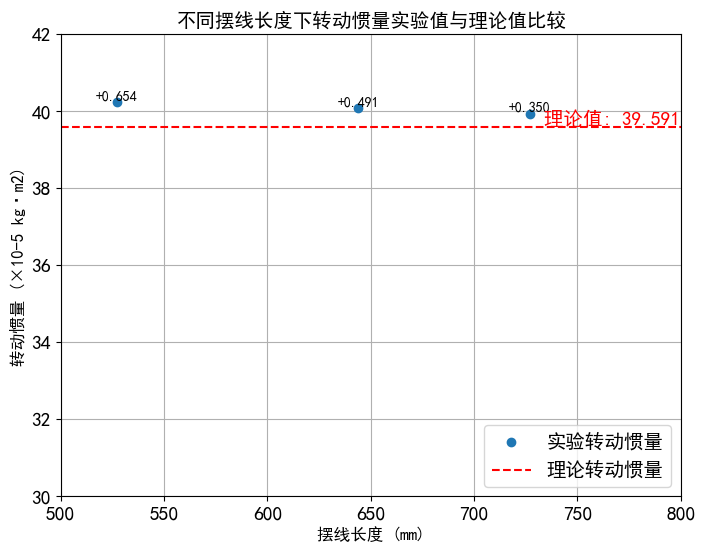
\includegraphics[width=\textwidth]{不同摆线长度下转动惯量实验值与理论值比较.png}
        \caption{不同摆线长度下转动惯量实验值与理论值比较}
        \label{fig:comparison_theory_experiment}
    \end{minipage}
    \hfill
    \begin{minipage}{0.48\textwidth}
        \centering
        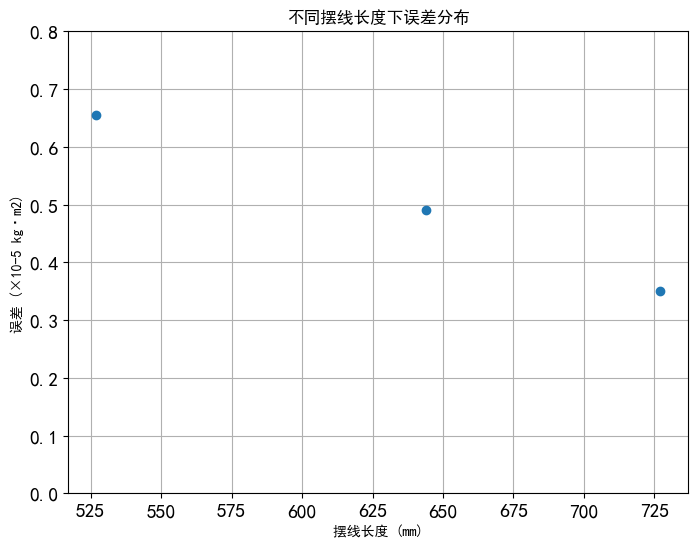
\includegraphics[width=\textwidth]{不同长度误差分布.png}
        \caption{不同长度误差分布}
        \label{fig:error_distribution}
    \end{minipage}
\end{figure}


\subsubsection{等效圆柱砝码的转动惯量测量}

根据平行轴定理,圆柱的转动惯量公式为:
$$
I = \frac{1}{8} m_s d_s^2 + m_s \left(\frac{s + d_s}{2}\right)^2
$$


其中,$m_s$ 为砝码质量,$d_s$ 为砝码直径,$s$ 为砝码间距。

实验测量数据如所示:
$m_s=79(g)$
,$d_s=18(mm)$,$g=9.8(m/s^2)$。


\begin{table}[h!]
    \centering
    \renewcommand{\arraystretch}{1.5}
    \setlength{\tabcolsep}{8pt}
    \begin{tabular}{|c|c|c|c|c|c|}
    \hline
    \multicolumn{6}{|c|}{\textbf{摆长为 727mm}} \\ \hline
    砝码间距$s$/mm & 10 & 20 & 30 & 40 & 50 \\ \hline
    摆动周期$T_1$/s & 1.014 & 1.147 & 1.302 & 1.462 & 1.648 \\ \hline
    摆动周期$T_2$/s & 1.020 & 1.122 & 1.302 & 1.658 & 1.652 \\ \hline
    平均周期$T$/s & 1.017 & 1.1345 & 1.302 & 1.660 & 1.650 \\ \hline
    \textbf{转动惯量/ $ \mathrm{10^{-5}kg \cdot m^2} $} & 1.86835 & 3.17185 & 4.87035 & 6.96385 & 9.45235 \\ \hline
    \end{tabular}
    \caption{摆长为 727mm 等效圆柱砝码的转动惯量测量数据}
    \label{tab:raw_data_simplified}
\end{table}

% 我现在需要一个表格,第一列标题为 No.,只有一行,第二列标题为摆长,只有一行,第三列标题空白,s 占一行,t 占两行,转动惯量 I 占一行,第四五六往后的列标题为 1,2,3,4,5,下面的内容为 3 行,


\begin{table}[h!]
    \centering
    \renewcommand{\arraystretch}{1.5}
    \setlength{\tabcolsep}{8pt}
    \begin{tabular}{|c|c|c|c|c|c|}
    \hline
    \multicolumn{6}{|c|}{\textbf{摆长为 464mm}} \\ \hline
    砝码间距$s$/mm & 10 & 20 & 30 & 40 & 50 \\ \hline
    摆动周期$T_1$/s & 0.819 & 0.928 & 1.056 & 1.168 & 1.318 \\ \hline
    摆动周期$T_2$/s & 0.818 & 0.924 & 1.053 & 1.172 & 1.328 \\ \hline
    平均周期$T$/s & 0.8185 & 0.926 & 1.0545 & 1.170 & 1.323 \\ \hline
    \textbf{转动惯量/ $ \mathrm{10^{-5}kg \cdot m^2} $} & 1.86835 & 3.17185 & 4.87035 & 6.96385 & 9.45235 \\ \hline
    \end{tabular}
    \caption{摆长为 464mm 等效圆柱砝码的转动惯量测量数据}
    \label{tab:raw_data_simplified}
\end{table}


\begin{figure}[h!]
    \centering
    \begin{minipage}{0.48\textwidth}
        \centering
        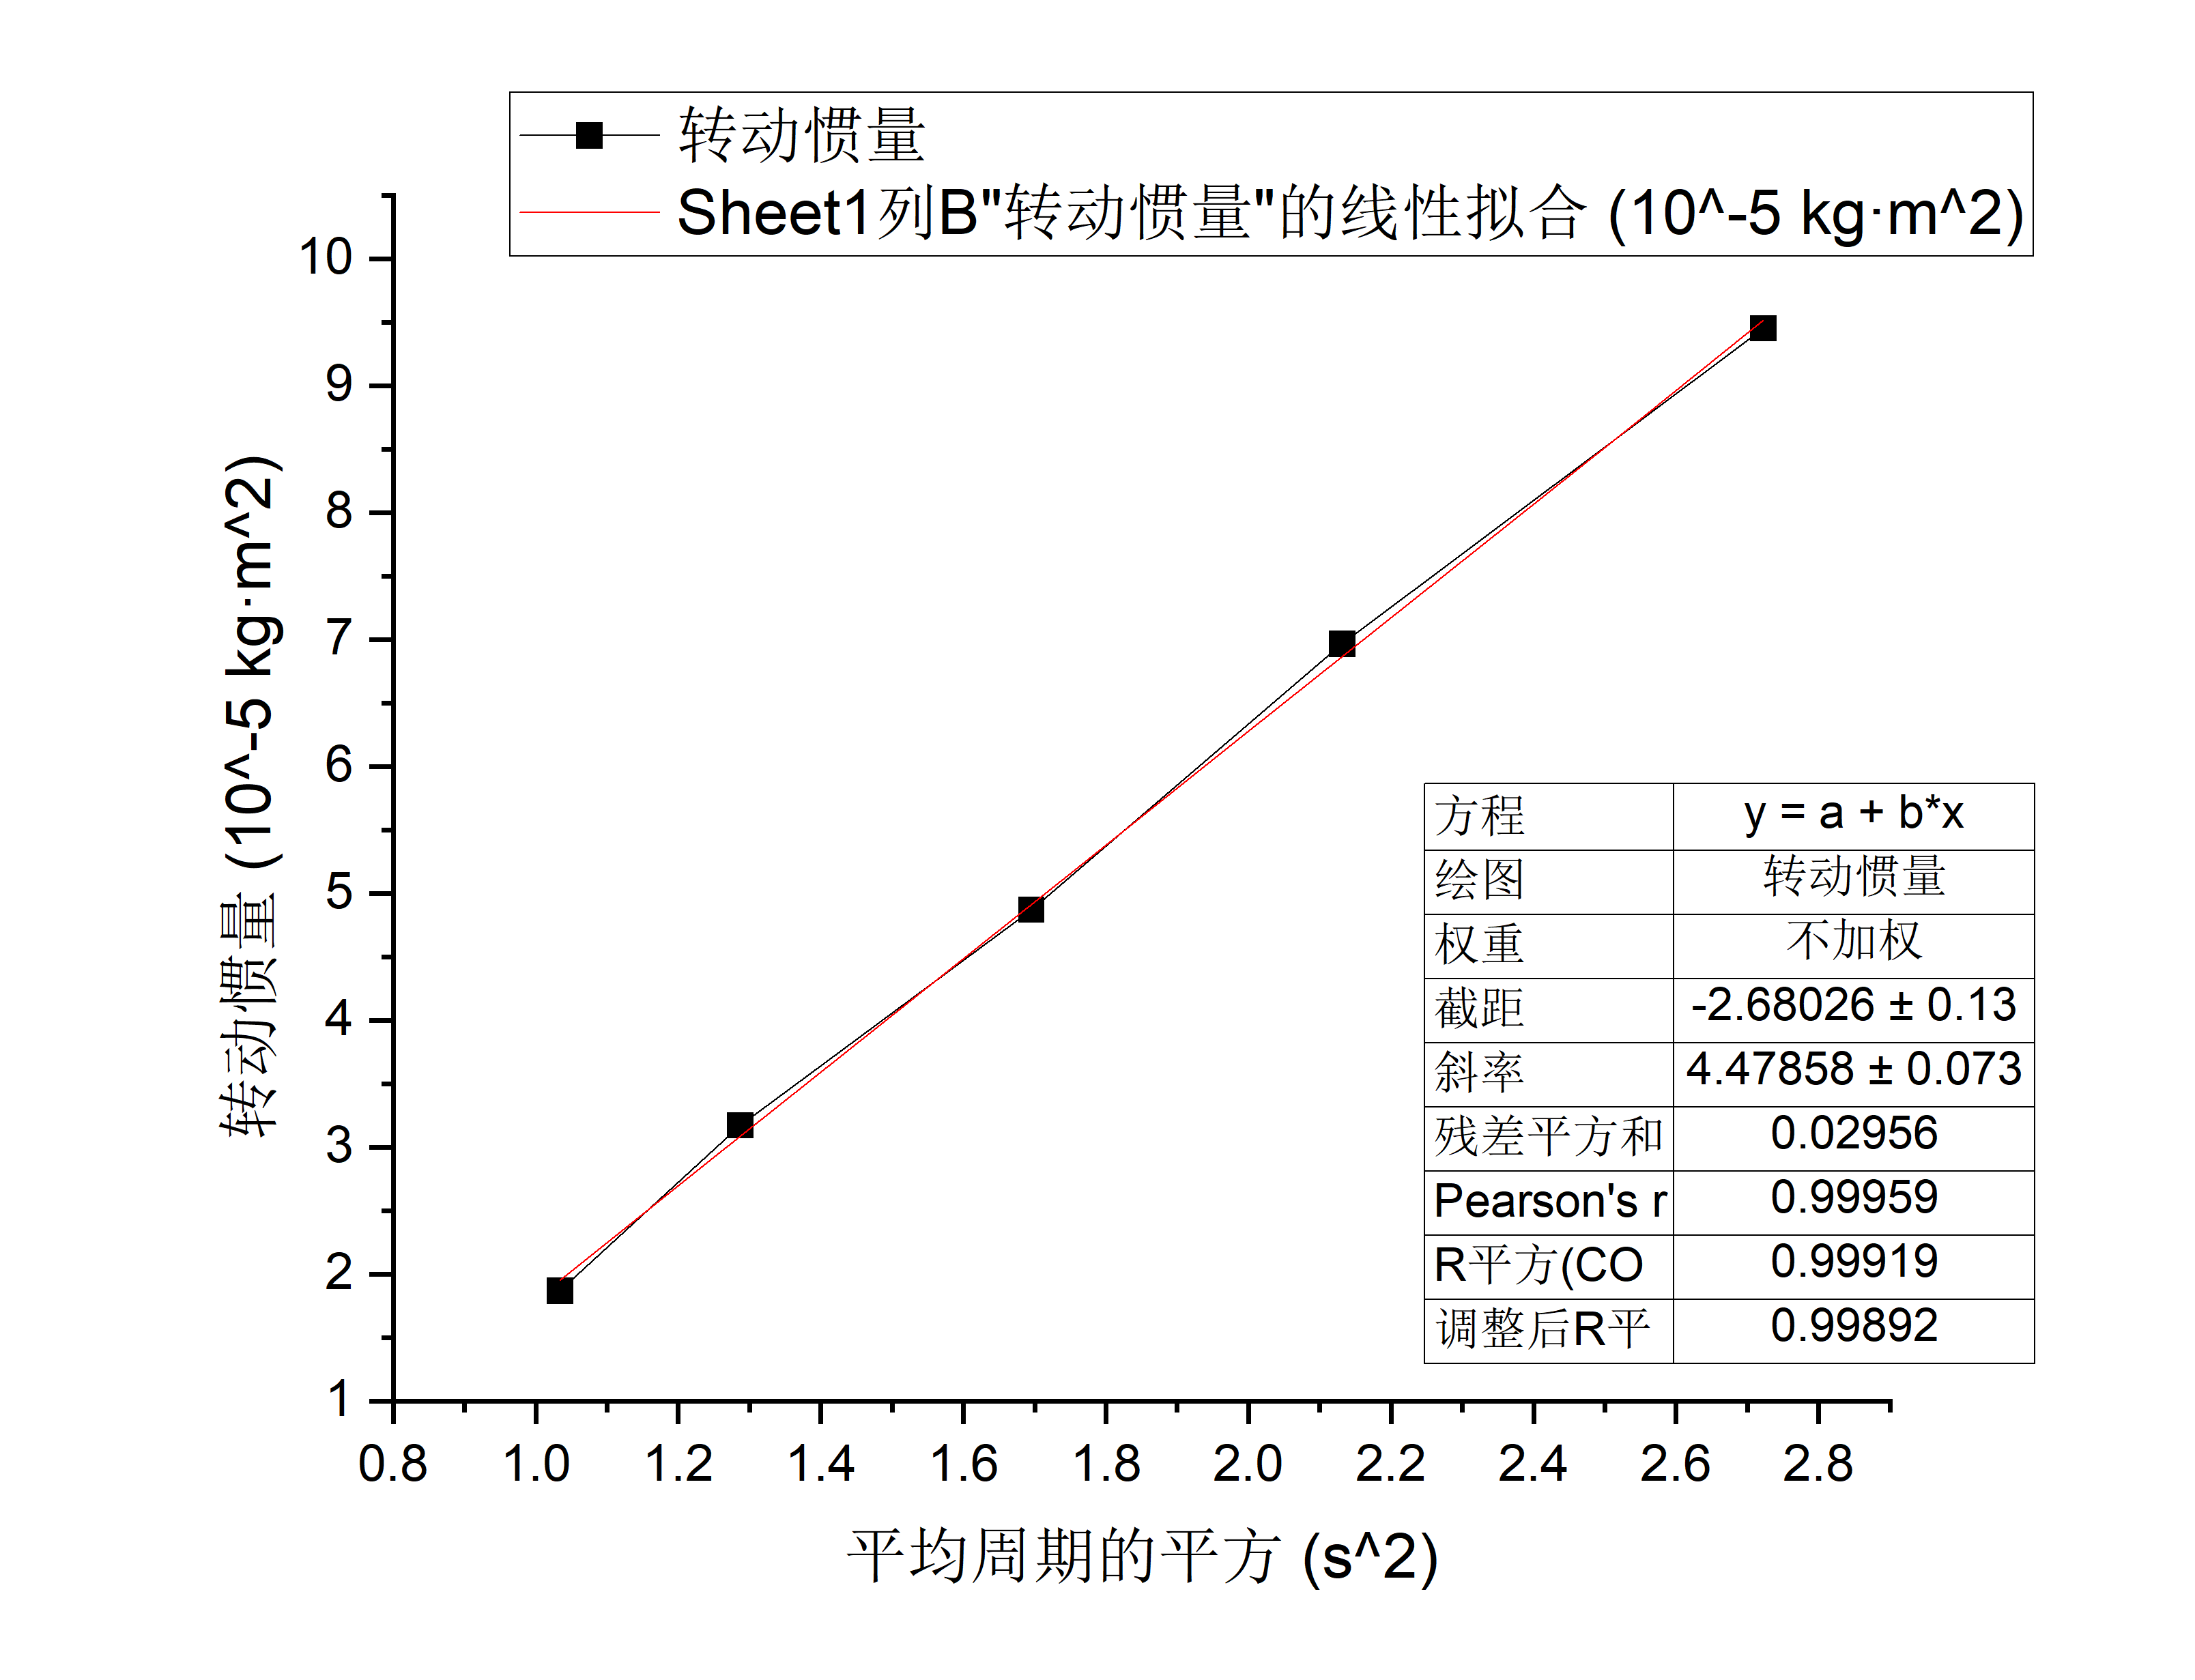
\includegraphics[width=\textwidth]{Young.png}
        \caption{摆长为 727mm 等效圆柱砝码的转动惯量测量数据}
        \label{fig:irregular_data_727}
    \end{minipage}
    \hfill
    \begin{minipage}{0.48\textwidth}
        \centering
        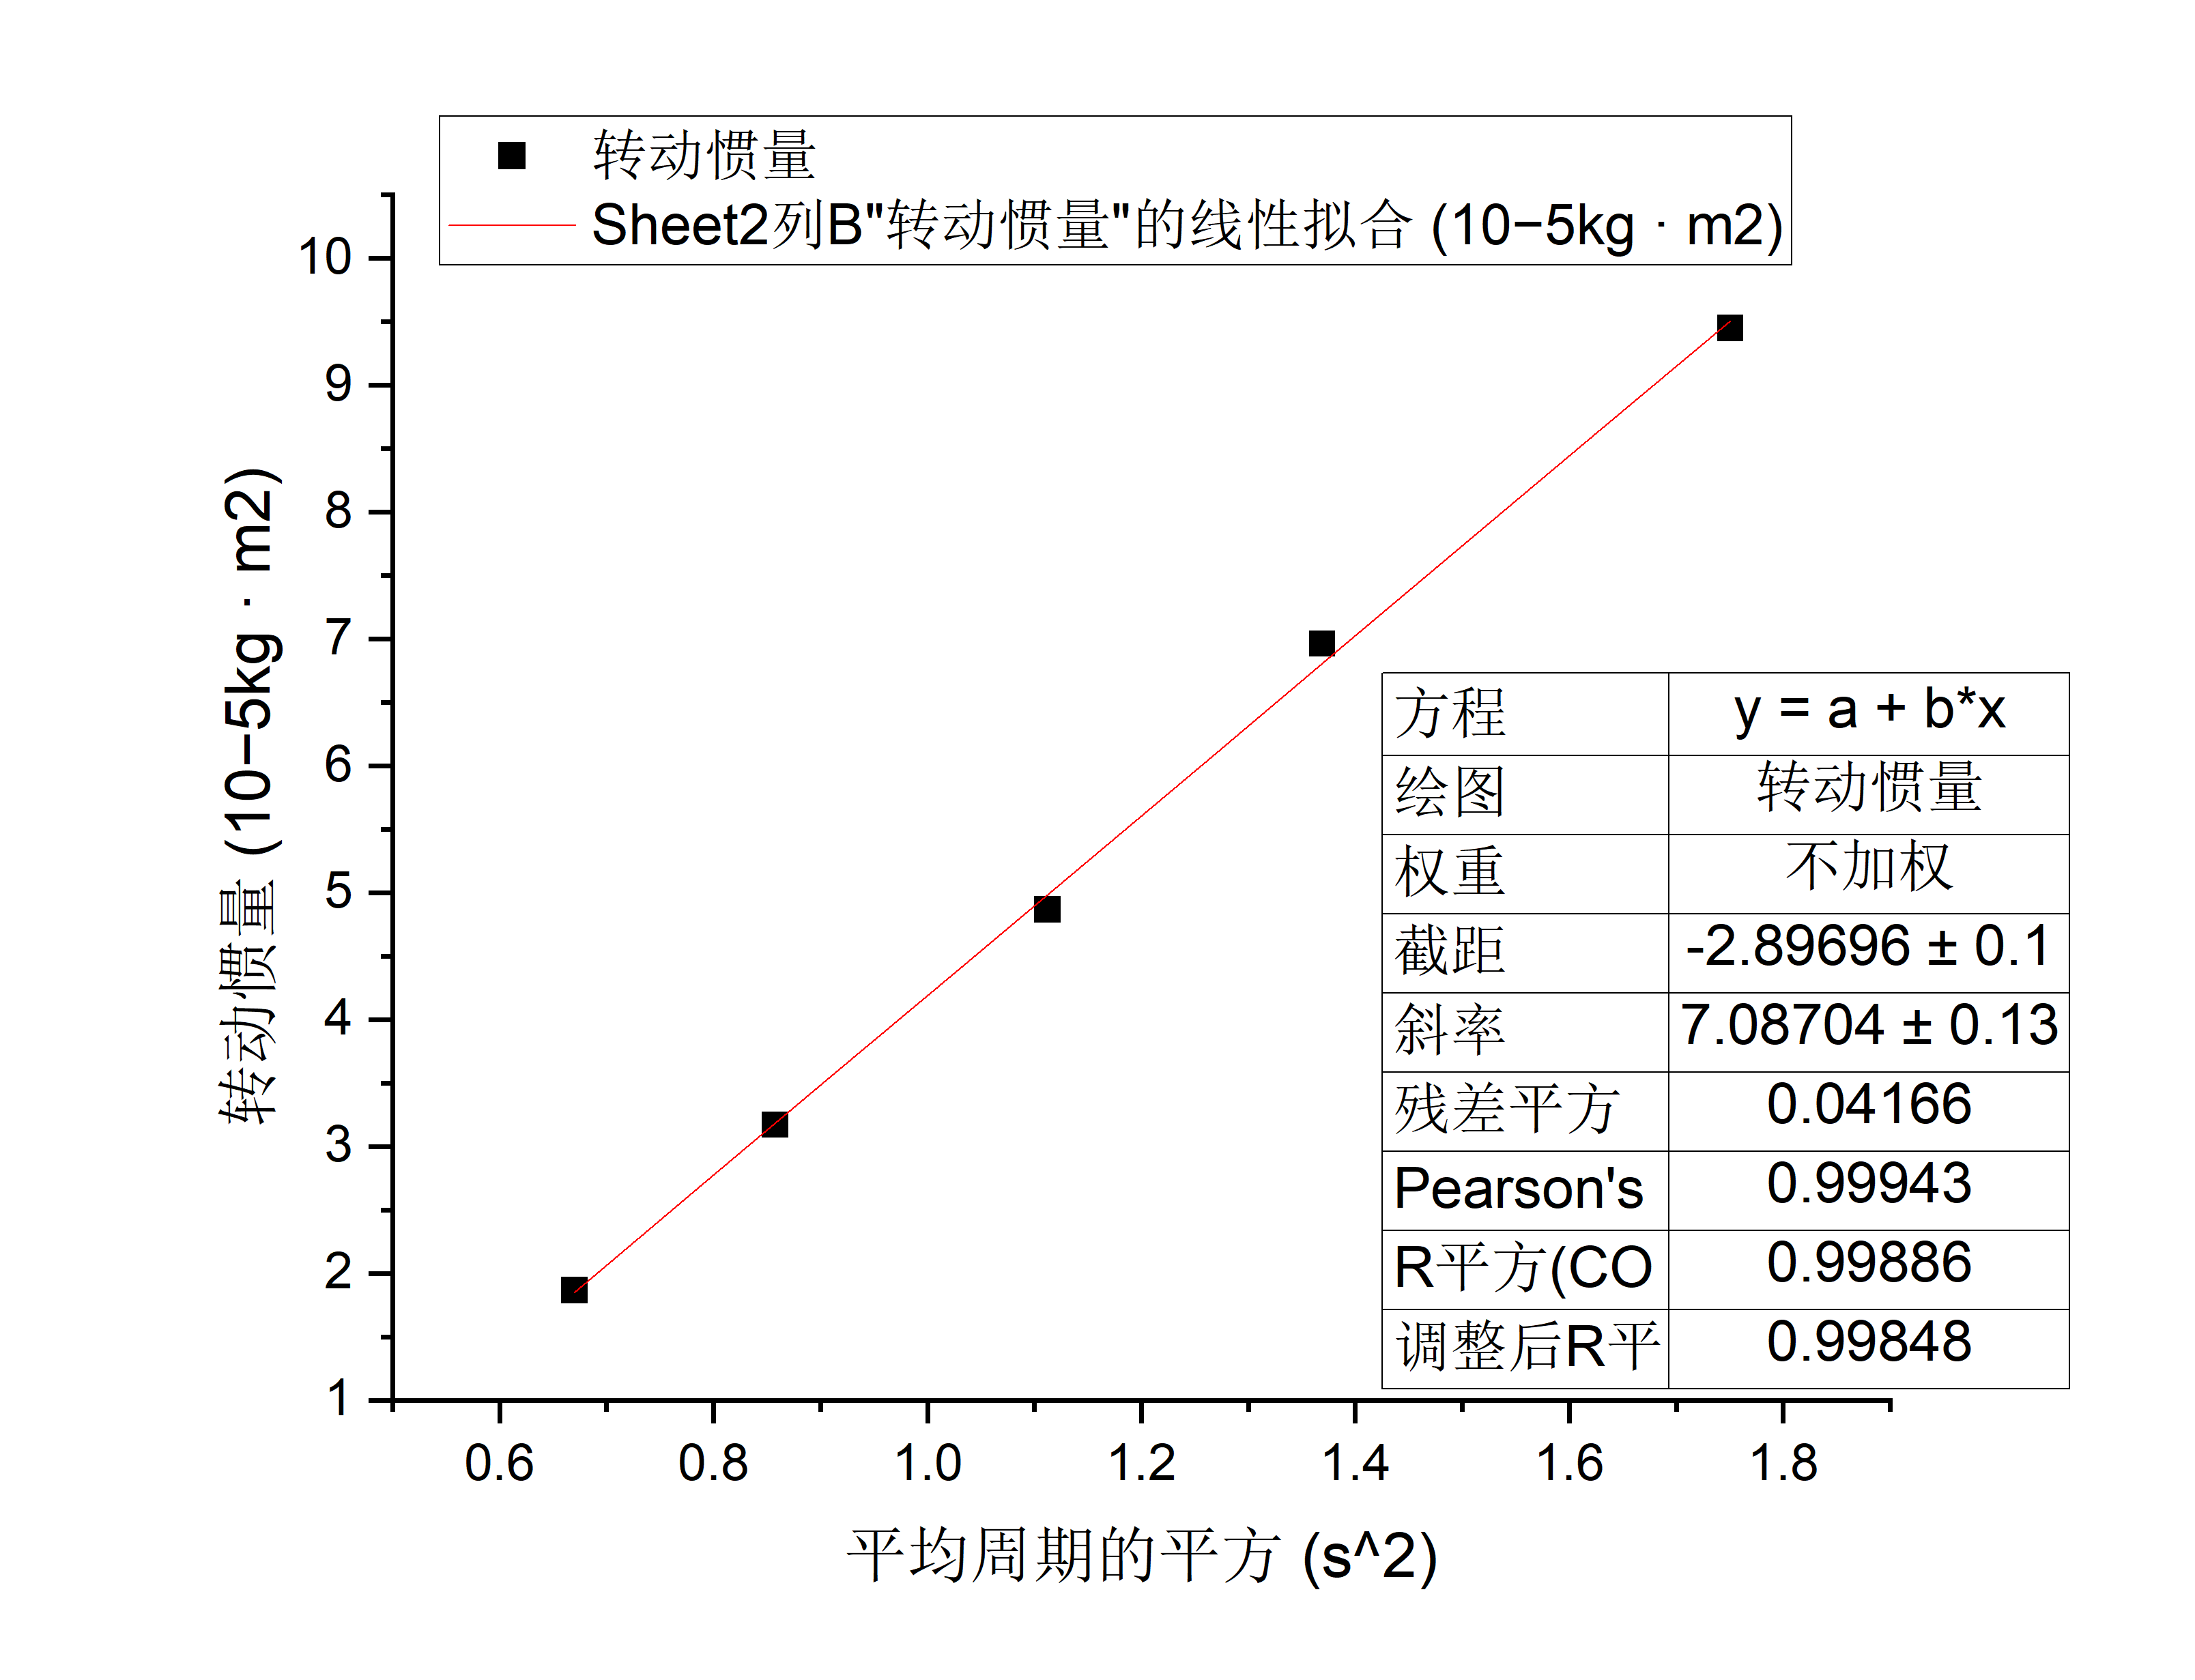
\includegraphics[width=\textwidth]{464.png}
        \caption{摆长为 464mm 等效圆柱砝码的转动惯量测量数据}
        \label{fig:irregular_data_464}
    \end{minipage}
\end{figure}

摆长为 464mm 回归方程为:
$$
I = 7.08704 \times T²  -2.8970
$$
得到
$$
I_1 = 7.08704 \times 1.048²  -2.8970=4.8867\times  \mathrm{10^{-5}kg \cdot m^2} 
$$
摆长为 727mm 回归方程为:
$$
I = 4.47858 \times T²  -2.8970
$$
得到
$$
I_2 = 4.47858 \times 1.048²  -2.68026=4.7072\times \mathrm{10^{-5}kg \cdot m^2} 
$$

\begin{figure}
    \centering
        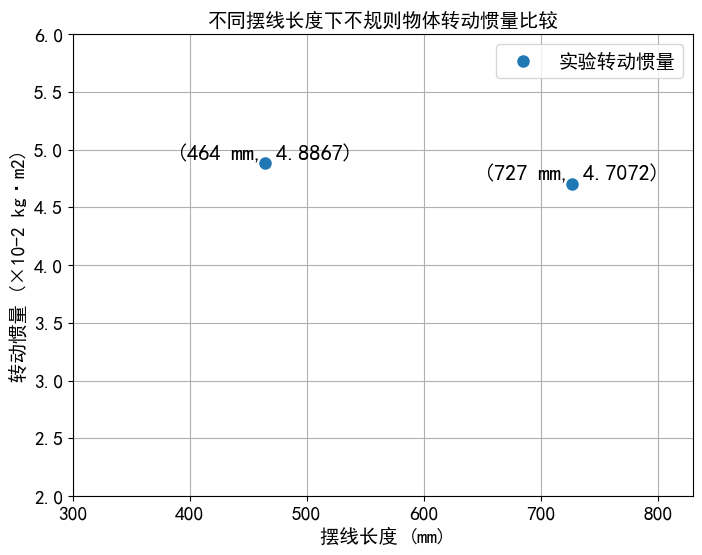
\includegraphics[width=0.5\textwidth]{不同摆线长度下不规则物体转动惯量比较.png}
        \caption{不同摆线长度下不规则物体转动惯量比较}
        \label{fig:irregular_data_464}
\end{figure}

\newpage
